\documentclass[english]{article}
\usepackage[english]{babel}
\usepackage{graphicx}
\usepackage{listings}
\usepackage{color}
\usepackage[utf8]{inputenc}

\definecolor{dkgreen}{rgb}{0,0.6,0}
\definecolor{gray}{rgb}{0.5,0.5,0.5}
\definecolor{mauve}{rgb}{0.58,0,0.82}

\lstset{frame=tb,
  language=Java,
  aboveskip=3mm,
  belowskip=3mm,
  showstringspaces=false,
  columns=flexible,
  basicstyle={\small\ttfamily},
  numbers=none,
  numberstyle=\tiny\color{gray},
  keywordstyle=\color{blue},
  commentstyle=\color{dkgreen},
  stringstyle=\color{mauve},
  breaklines=true,
  breakatwhitespace=true,
  tabsize=3
}


\title{%
  Chess Game with CPU Opponent \\
  \large Advanced Computer Programming Project}

\begin{document}
\maketitle

\section{Introduction}
The goal of this project is to code a Chess Game in order to let the human player play against a CPU opponent which uses the minimax algorithm.

\subsection{Minimax Algorithm}
The minimax algorithm is a simple algorithm that allows the CPU opponent to choose which move to make in many different games.

It's very similar to a brute force technique: it constructs a tree of moves with n-depth, and chooses which is the best move to make in order to gain more advantage.

When the end of the tree (maximum depth) is reached it starts exploring the tree backwards:
\begin{enumerate}
	\item If it's its turn it will choose the move which will give it the maximum advantage
	\item If it's opponent turn it will choose the move which will give to the opponent the maximum advantage
\end{enumerate}

These two steps are repeated for every layer of the tree, at the end it will remain only one value (which identifies one move).

An example can be seen in Figure \ref{fig:minimax}.

\begin{figure}
 	\centering
  	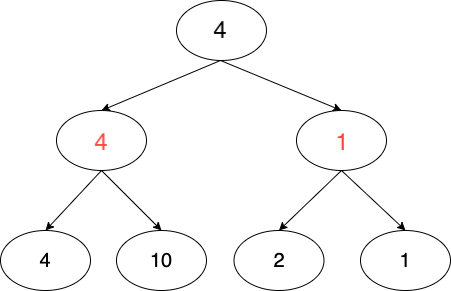
\includegraphics[width=200px]{img/minimax.png}
 	 \label{fig:minimax}
 	 \caption{Minimax example}
\end{figure}

In order to evaluate the moves I assigned the following values to pieces:

\begin{itemize}
	\item Pawn: 1
	\item Knight: 3
	\item Bishop: 3
	\item Rook: 5
	\item Queen: 9
\end{itemize}

The move evaluation is done as follows:

Value of piece that will be eaten * 2 - Value of piece that will eat it

+ 10 (if that move puts the opponent's king in check) 

+  1000 (if that move puts the opponent's king in checkmate)

\section{Implementation}
I used Python 3.8 to implement the application, with TkInter as GUI.
In the implementation I've chosen to use the following advanced computer programming techniques:
\begin{itemize}
	\item Object Oriented Programming
	\item Concurrent Programming	
	\item Functional Programming
\end{itemize}

\subsection{Object Oriented Programming}
The Object Oriented Programming part is used in every part of the project, there are several classes used in it.
The most interesting part is the definition of the Chess Pieces, because it particularly lends to the definition of Object Oriented Programming.

The pieces were implemented at first by defining a  "Piece" class which is the base class for all the different Pieces.
The class is defined as follows:

\begin{lstlisting}
#Pieces.py

class Piece:
        
    def move (self,nrow,ncol):
        self.row = nrow
        self.col = ncol

    def get_col_letter (self):
        letters[8] = ['A','B','C','D','E','F','G','H']
        return letters[self.col];

    def get_col (self):
        return self.col
    
    def get_row (self):
        return self.row
    
    def get_color (self):
        return self.color

    def get_image_path (self):
        return self.image

    def get_val (self):
        return self.val

    def get_moves_path (self,row_func,col_func,board):
        moves = []
        for i in range(1,9):
            if (self.can_move(row_func(self.row,i),col_func(self.col,i))):
                if (board.get_piece(row_func(self.row,i),col_func(self.col,i)) == None):
                    moves.append((row_func(self.row,i),col_func(self.col,i)))
                elif (board.get_piece(row_func(self.row,i),col_func(self.col,i)) != None and board.get_piece(row_func(self.row,i),col_func(self.col,i)).get_color() != self.get_color()):
                    moves.append((row_func(self.row,i),col_func(self.col,i)))
                    break
                else:
                    break
            else:
                break
        return moves

    def __init__ (self,row,col,id,val,color):
        self.row = row
        self.col = col
        self.id = id
        self.val = val
        self.color = color
\end{lstlisting}

All the methods that we can see in this class will then be available in any inherited class with this class as base class.
One example of inherited class could be the Queen's class:

\begin{lstlisting}
#Pieces.py

class Queen (Piece):
    
    def type (self): 
        return 'queen'

    def short_type (self):
        return 'q'

    def can_move(self,nrow,ncol): 
        if ((nrow <= 8 and ncol <= 8 and nrow >= 1 and ncol >= 1) and ((self.get_col() == ncol) or (self.get_row() == nrow) or (abs(self.get_row() - nrow) == abs(self.get_col() - ncol)))):
            return True
        return False

    def get_moves (self,board,king = None):
        temp_moves = []
        moves = []
        for x in self.get_moves_path(lambda row, i: row + i,lambda col, i: col,board):
            temp_moves.append(x)
        for x in self.get_moves_path(lambda row, i: row,lambda col, i: col + i,board):
            temp_moves.append(x)
        for x in self.get_moves_path(lambda row, i: row - i,lambda col, i: col,board):
            temp_moves.append(x)
        for x in self.get_moves_path(lambda row, i: row,lambda col, i: col - i,board):
            temp_moves.append(x)
        for x in self.get_moves_path(lambda row, i: row + i,lambda col, i: col + i,board):
            temp_moves.append(x)
        for x in self.get_moves_path(lambda row, i: row + i,lambda col, i: col - i,board):
            temp_moves.append(x)
        for x in self.get_moves_path(lambda row, i: row - i,lambda col, i: col + i,board):
            temp_moves.append(x)
        for x in self.get_moves_path(lambda row, i: row - i,lambda col, i: col - i,board):
            temp_moves.append(x)
        if king != None:
            for move in temp_moves:
                temp_board = copy.deepcopy(board)
                temp_board.move(self.get_row(),self.get_col(),move[0],move[1])
                if (not(king.is_in_check(temp_board))):
                    moves.append(move)
            return moves
        return temp_moves

    def __init__ (self,row,col,id,color):
        super().__init__(row,col,id,9,color)
        if (self.color == 'b'):
            self.image = "img/blackq.png"
        else:
            self.image = "img/whiteq.png"
\end{lstlisting}

As we can see in the class there are other implemented methods (besides the ones in the base class) defined differently for every other Chess Pieces such as Rook, Knight, Pawn, King and Bishop.

The inheritance in this case is very useful because it allows to define some base methods which otherwise must have been defined for every single class. 

\subsection{Concurrent Programming}
The minimax algorithm is computationally expensive, as it has to see at n-depth all the possible moves on the board.
In order to reduce the waiting time for the CPU to make the move I chose to adopt the multithreading programming in two different points:
\begin{itemize}
	\item Getting all the possible moves for a piece (one thread for each piece)
	\item Evaluate the value of a move with minimax algorithm (one thread for each possible moves)
\end{itemize}

In Python we can implement the multithread making a class which inherits threading.Thread.
The class must contain a run() method which will contain the instructions to be executed when the thread will be run.
The thread which gets a piece's moves is implemented as follows:

\begin{lstlisting}
#Threads.py

class GetMovesThread (threading.Thread):

    def run (self):
        self.moves = []
        for move in self.piece.get_moves(self.chess,self.chess.get_king(self.piece.get_color())):
            self.moves.append(Move(self.piece.get_row(),self.piece.get_col(),move[0],move[1],self.chess.move_eval((self.piece.get_row(),self.piece.get_col()),(move[0],move[1]))))

    def __init__ (self,name,piece,chess):
      threading.Thread.__init__(self)
      self.name = name
      self.piece = piece
      self.chess = chess

\end{lstlisting}

This thread is called with:

\begin{lstlisting}
#Chess.py

def get_possible_moves (self,color):
        moves = []
        threads = []
        for cell in self.chess_grid:
            if (cell != None and cell.color == color):
                thread = GetMovesThread("Thread minimax",cell,self)
                thread.start()
                threads.append(thread)
        for thread in threads:
            thread.join()
        for thread in threads:
            for move in thread.moves:
                moves.append(move)
        return moves

\end{lstlisting}

In the first part the two lists (moves and threads) are initialized, with a "for" cycle every piece on the board is analyzed and for that piece a thread is started.
Then we wait for all the threads to finish with the second "for" cycle and a list with moves is returned.

The other multithread part is the minimax algorithm, implemented as follows:

\begin{lstlisting}
#Threads.py

class MinimaxThread (threading.Thread):

    def run (self):
        self.result = self.minimax(1,self.chess,self.move,self.color)

    def minimax (self,depth,chess,move,color):
        temp_chess = copy.deepcopy(chess)
        temp_chess.move(move.move_from[0],move.move_from[1],move.move_to[0],move.move_to[1])
        if (depth == 0): return move.val
        else:
            if (color == 'b'):
                moves = temp_chess.get_possible_moves('b')
                if (len(moves) == 0):
                    return move.val
                moves_values = map(self.minimax,[depth-1]*len(moves),[temp_chess]*len(moves),moves,['w']*len(moves))
                return max(moves_values)
            else:
                moves = temp_chess.get_possible_moves('w')
                if (len(moves) == 0):
                    return move.val
                moves_values = map(self.minimax,[depth-1]*len(moves),[temp_chess]*len(moves),moves,['w']*len(moves))
                return min(moves_values)

    def __init__ (self,name,chess,move,color):
      threading.Thread.__init__(self)
      self.name = name
      self.chess = chess
      self.move = move
      self.color = color
\end{lstlisting}

And it is called as follows:

\begin{lstlisting}
#Ai.py

def choose_move (self):
        threads = []
        moves = self.chess.get_possible_moves('b')
        random.shuffle(moves)
        for move in moves:
            thread = MinimaxThread("Thread minimax",copy.deepcopy(self.chess),move,'w')
            thread.start()
            threads.append(thread)
        for thread in threads:
            thread.join()
        best_move = None
        for thread in threads:
            if (best_move == None or thread.result >= best_move.val):
                best_move = thread.move
        return best_move
\end{lstlisting}

The workflow of this code is similar to the one we saw before, the only different part is the check on the result of the moves.

The choice to use Concurrent Programming with multi threading was dictated by the fact that these algorithms are computationally expensive, inserting multi threading in these parts of code will make the application more efficient.

\subsection{Functional Programming}
The functional programming is used in different parts of the project, it is used in order to get the possible moves for different pieces: Queen, Bishop, Tower.
In order to get the moves it was written a method in the "Piece" class:

\begin{lstlisting}
#Pieces.py

def get_moves_path (self,row_func,col_func,board):
        moves = []
        for i in range(1,9):
            if (self.can_move(row_func(self.row,i),col_func(self.col,i))):
                if (board.get_piece(row_func(self.row,i),col_func(self.col,i)) == None):
                    moves.append((row_func(self.row,i),col_func(self.col,i)))
                elif (board.get_piece(row_func(self.row,i),col_func(self.col,i)) != None and board.get_piece(row_func(self.row,i),col_func(self.col,i)).get_color() != self.get_color()):
                    moves.append((row_func(self.row,i),col_func(self.col,i)))
                    break
                else:
                    break
            else:
                break
        return moves
\end{lstlisting}

This method applies row\_func and col\_func to a certain piece repeatedly until it found a piece interrupting the path (or the end of the board is reached).
As it is written it accept as input two different functions, this is because the movement for the pieces we talked above are different.
We can see how this method is used for the three different pieces:

\begin{lstlisting}
#Pieces.py

#Queen
def get_moves (self,board,king = None):
        temp_moves = []
        moves = []
        for x in self.get_moves_path(lambda row, i: row + i,lambda col, i: col,board):
            temp_moves.append(x)
        for x in self.get_moves_path(lambda row, i: row,lambda col, i: col + i,board):
            temp_moves.append(x)
        for x in self.get_moves_path(lambda row, i: row - i,lambda col, i: col,board):
            temp_moves.append(x)
        for x in self.get_moves_path(lambda row, i: row,lambda col, i: col - i,board):
            temp_moves.append(x)
        for x in self.get_moves_path(lambda row, i: row + i,lambda col, i: col + i,board):
            temp_moves.append(x)
        for x in self.get_moves_path(lambda row, i: row + i,lambda col, i: col - i,board):
            temp_moves.append(x)
        for x in self.get_moves_path(lambda row, i: row - i,lambda col, i: col + i,board):
            temp_moves.append(x)
        for x in self.get_moves_path(lambda row, i: row - i,lambda col, i: col - i,board):
            temp_moves.append(x)
        if king != None:
            for move in temp_moves:
                temp_board = copy.deepcopy(board)
                temp_board.move(self.get_row(),self.get_col(),move[0],move[1])
                if (not(king.is_in_check(temp_board))):
                    moves.append(move)
            return moves
        return temp_moves
        
#Bishop
def get_moves (self,board,king = None):
        temp_moves = []
        moves = []
        for x in self.get_moves_path(lambda row, i: row + i,lambda col, i: col + i,board):
            temp_moves.append(x)
        for x in self.get_moves_path(lambda row, i: row + i,lambda col, i: col - i,board):
            temp_moves.append(x)
        for x in self.get_moves_path(lambda row, i: row - i,lambda col, i: col + i,board):
            temp_moves.append(x)
        for x in self.get_moves_path(lambda row, i: row - i,lambda col, i: col - i,board):
            temp_moves.append(x)
        if king != None:
            for move in temp_moves:
                temp_board = copy.deepcopy(board)
                temp_board.move(self.get_row(),self.get_col(),move[0],move[1])
                if (not(king.is_in_check(temp_board))):
                    moves.append(move)
            return moves
        return temp_moves
        
#Rook
def get_moves (self,board,king = None):
        temp_moves = []
        moves = []
        for x in self.get_moves_path(lambda row, i: row + i,lambda col, i: col,board):
            temp_moves.append(x)
        for x in self.get_moves_path(lambda row, i: row,lambda col, i: col + i,board):
            temp_moves.append(x)
        for x in self.get_moves_path(lambda row, i: row - i,lambda col, i: col,board):
            temp_moves.append(x)
        for x in self.get_moves_path(lambda row, i: row,lambda col, i: col - i,board):
            temp_moves.append(x)
        if king != None:
            for move in temp_moves:
                temp_board = copy.deepcopy(board)
                temp_board.move(self.get_row(),self.get_col(),move[0],move[1])
                if (not(king.is_in_check(temp_board))):
                    moves.append(move)
            return moves
        return temp_moves
\end{lstlisting}

As we can see we pass the functions we need for rows and columns as arguments to get\_moves\_path method.

In this case the use of functional programming has been dictated to the fact that the the way to get the moves for those pieces was very similar between them, and writing the same code different times was a bad engineering choice; the use of lambdas and functions passed as argument to other functions adapts perfectly to this case.

Another use of functional programming can be found in the minimax algorithm:

\begin{lstlisting}
#Threads.py

def minimax (self,depth,chess,move,color):
        temp_chess = copy.deepcopy(chess)
        temp_chess.move(move.move_from[0],move.move_from[1],move.move_to[0],move.move_to[1])
        if (depth == 0): return move.val
        else:
            if (color == 'b'):
                moves = temp_chess.get_possible_moves('b')
                if (len(moves) == 0):
                    return move.val
                moves_values = map(self.minimax,[depth-1]*len(moves),[temp_chess]*len(moves),moves,['w']*len(moves))
                return max(moves_values)
            else:
                moves = temp_chess.get_possible_moves('w')
                if (len(moves) == 0):
                    return move.val
                moves_values = map(self.minimax,[depth-1]*len(moves),[temp_chess]*len(moves),moves,['w']*len(moves))
                return min(moves_values)
\end{lstlisting}

The functional programming is used in the map function: a function that maps a certain function to all the elements of a list; in this case we need the map to apply the minimax algorithm to all the moves we got.
Another example of functional programming is in the return of the method: the code gets the best value simply by applying the max and the min functions to the list with the computed values.

I chose to use functional programming in this part of the code because it makes the code much more readable and compact, and also because the intensive use of lists of moves is very synergistic with the functional programming's functions.

\end{document}